\documentclass[15pt]{extarticle}

\usepackage{geometry}
\usepackage{pdflscape}
\geometry{
	a4paper,
	total={170mm,257mm},
	left=10mm,
	top=20mm,
	right=10mm,
	bottom=20mm
}
\usepackage[dvipsnames]{xcolor}
\usepackage[utf8]{inputenc}
\usepackage[bulgarian]{babel}
\usepackage{amsfonts}
\usepackage{amsmath}
\usepackage{endnotes}
\usepackage[normalem]{ulem}
\usepackage[framemethod=tikz]{mdframed}
\usepackage[hidelinks]{hyperref}
\usepackage{titling}
\usepackage{fancyhdr}
\usepackage{listings}
\pagestyle{fancy}
\lhead{\copyright Калоян Цветков}
\rhead{Интерпретатор на \emph{Prolog}}
\renewcommand{\headrulewidth}{0.4pt}
\renewcommand{\footrulewidth}{0.4pt}

\newcommand{\version}{1.0.0}

\usepackage{listings}
\usepackage{color}

\definecolor{dkgreen}{rgb}{0,0.6,0}
\definecolor{gray}{rgb}{0.5,0.5,0.5}
\definecolor{mauve}{rgb}{0.58,0,0.82}

\lstset{frame=tb,
	aboveskip=3mm,
	belowskip=3mm,
	showstringspaces=false,
	columns=flexible,
	basicstyle={\large\ttfamily},
	numbers=none,
	numberstyle=\tiny\color{red},
	keywordstyle=\color{blue},
	commentstyle=\color{dkgreen},
	stringstyle=\color{mauve},
	breaklines=true,
	breakatwhitespace=true,
	tabsize=3
}

\title{\Huge Документация към проект\\ \huge Интерпретатор на \emph{Prolog}\\ \large ФП, зимен семестър 2022/2023}
\author{Калоян Цветков\\ \texttt{4MI0800017}}
\date{ФМИ, СУ\\ \version}

\begin{document}
	
	\begin{titlingpage}
		\maketitle
	\end{titlingpage}
	\tableofcontents
	\newpage
	\large
	
	\section{Кратко описание}
	
	Интерпретаторът е написан на езика Haskell и компилиран чрез GHC, версия $8.10.7$.\\
	Може да определя истинността на факти, заредени от програма на езика \emph{Prolog}, използвайки директно записаните в него константни факти или използвайки изводи от правила.\\
	При подаване на факт, съдържащ променлива (заявка), интерпретаторът определя всички стойности на променливата, за които фактът е верен (ако има такива според кода) и при поискване ги принтира. Също така може да разрешава равенства не термове, отново посочвайки за кои стойности на променливите равенството е изпълнено.\\
	Интерпретаторът е изпълним файл, който се стартира в конзола.
	
	\section{Структура}
	
	Сорс-кодът е разделен в 8 модула:
	\begin{itemize}
		
		\item \textbf{\texttt{Prolog}}
		
		Съдържа всички останали модули;
		
		\item \textbf{\texttt{Datatypes}}
		
		Съдържа всички потрбителски типове, представляващи елементите на една програма на \emph{Prolog};
		
		\item \textbf{\texttt{Checkers}}
		
		Предикати, определящи дали низ може да се конвертира до синтактичен елемент от \emph{Prolog} и други;
		
		\item \textbf{\texttt{Conversions}}
		
		Функции за конвертиране между синтактични елементи на \emph{Prolog};
		
		\item \textbf{\texttt{Identities}}
		
		Функции за проверка на идентичност на потребителски типове;
		
		\item \textbf{\texttt{Tools}}
		
		Общи функции за обработка на данни;
		
		\item \textbf{\texttt{Unification}}
		
		Реализация на алгоритъма за унификация на термове
		
		\item \textbf{\texttt{Resolutions}}
		
		Основен метод; съдържа функции за проверка на истинност на факти.
		
	\end{itemize}

	Файлът \textbf{\texttt{main.hs}} съдържа само функции за работа с външния свят (вход и изход).
	
	\section{Основни концепции и функции}
	
	\subsection{Примерен входен файл}
	
	Входен файл: \emph{prolog/starwars.pl}:
	
	\begin{lstlisting}[language=Prolog,numbers=right]
		%father/2
		father(ruwee, padme).
		father(anakin, luke).
		father(anakin, leia).
		father(han, ben).
		
		%mother/2
		mother(jobal, padme).
		mother(shmi, anakin).
		mother(padme, luke).
		mother(padme, leia).
		mother(leia, ben).
		
		%alias/2
		alias(darthvader, anakin).
		alias(kyloren, ben).
		alias(X,Y) :- alias(Y,X).
		
		%parent/2
		parent(X,Y) :- father(X, Y).
		parent(X,Y) :- mother(X, Y).
		
		%parent/2
		childof(X,Y) :- parent(Y,X).
	\end{lstlisting}
	
	\subsection{Унификация на термове}
	
	За унификация на два терма се грижи функцията
	
	\begin{lstlisting}[language=haskell]
		toBeUnified :: (Term, Term) -> QueryResult
	\end{lstlisting}
	
	Фунцкията имплементира следния алгоритъм за унификация:
	
	\begin{lstlisting}[numbers=right]
		Input: Terms A, B
		Initialize the result list to be empty;
		Initialize the stack with pair (A,B);
		Initialize the fail flag to false;
		While stack is not empy and not fail do:
		pop (X,Y) from the stack
		Case
		X is a variable:
		Substitute X with Y in the stack
		add X=Y to the list
		Y is a variable:
		Substitute Y with X in the stack
		add Y=X int the list
		X and Y are identical constants 
		continue
		X is atom f(X_1,...,X_n) and Y is atom f(Y_1,...,Y_n) for some identifier f and n>0:
		for i=1...n: push (X_i,Y_i) in the stack
		otherwise:
		set fail to true
		end Case
		end While
		Output:
		If fail, then empty QueueResult
		else QueryResult, corresponding to the result list;
		
	\end{lstlisting}

	\begin{landscape}
	
	\subsection{Резолюция}
	
	Резолюцията на термове се извършва по алгоритъма на \emph{SLD резолюцията}. Строи се кореново дърво, чиито върхове съдържат (на практика не е необходимо) конюнкция на термове. Листата на дървото съдържат необходими преобразувания до достигане на верен факт от заявката. Дървото е потенциално безкрайно, но благодарение на механизма за нормално оценяване, самото конструиране на дървото и извличане на резултати от него стават паралелно.

	\subsubsection{Примерно дърво}
	
	 Заявката е \emph{"parent(Parent,Child)"}:
	
	\begin{center}
		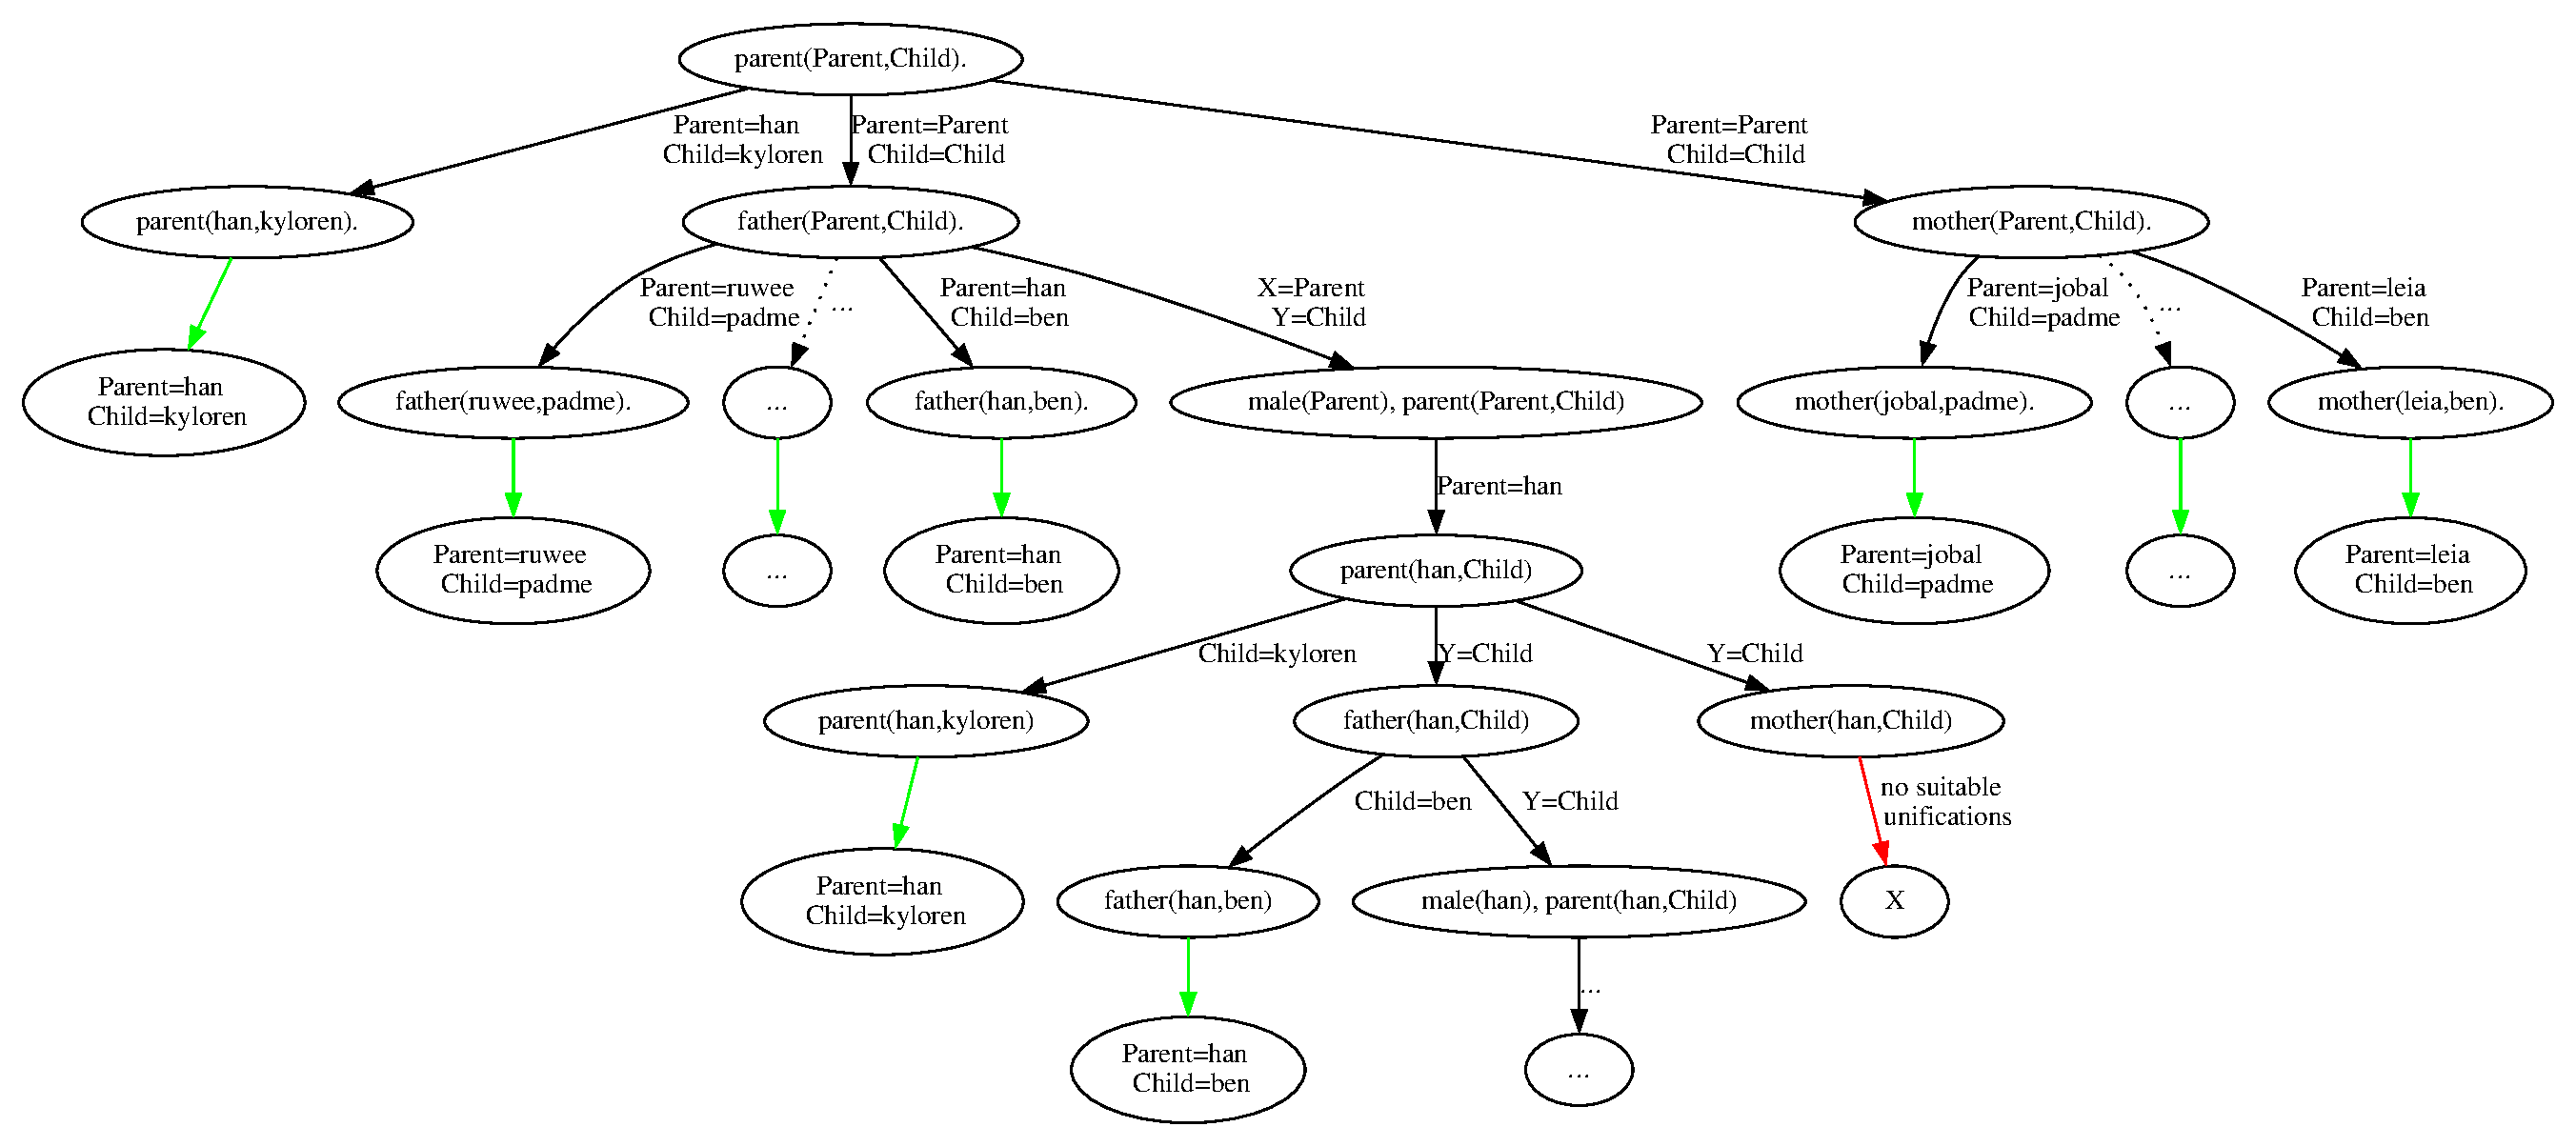
\includegraphics[scale=.58]{assets/rTree.eps}
	\end{center}
	
	\end{landscape}
	
	\section{Работа с приложението}
	
	\subsection{Начин на работа}
	
	След стартиране, приложението изисква да се въведе от клавиатурата път до код на \emph{Prolog}. При въведен синтактично неправилен низ или път, който не води към файл, приложенито пита повторно дали потребителят желае да въведе нов път. Ако пътят е валиден, всички факти в него биват проверени за синтактична вярност и се изписва съобщение с резултата (неверните редове биват изведени и в последствие не биват разглеждани).\\
	След това започва \emph{Read-Eval-Print-Loop}, очакващ потребителят да въведе равенство, факт или заявка, и съответно интерпретаторът изписва резултатите.\\
	Работата с текущия файл приключва след подаване на команда \emph{quit}.
	
	\subsection{Примерна работа}
	
	Стартиране на интерпретатора (в конзолен режим):
	
	%todo edit
	\begin{lstlisting}
		Which file to consult from the directory "prolog/"?
		> starwar.pl
		No such file...
		Consult another file? ( y | [n] )
		> y
		Which file to consult from the directory "prolog/"?
		> starwars.pl
		true.
		> father(anakin,luke).
		true.
		> father(anakin,luke)
		You are allowed to input only facts, queries and equalities!
		> father(luke,anakin).
		false.
		> father(Parent,Child).
		Parent = ruwee.
		Child = padme.
		
		Parent = anakin.
		Child = luke.
		
		Parent = anakin.
		Child = leia.
		
		Parent = han.
		Child = ben.
		
		Parent = han.
		Child = kyloren.
		.
		> a(X)=a(arg).
		X = arg.
		> a(Y,r)=b(X,Z).
		false.
		> a(Y,r)=a(X,Z).
		Y = X.
		Z = r.
		> pred(Z,Z)=pred(X,t).
		X = t.
		Z = t.
		> pred(Z,Z)=pred(X,Y).
		Y = X.
		Z = Y.
		> quit
		Consult another file? ( y | [n] )
		> no
		Closing...
		
	\end{lstlisting}
	
	
\end{document}